\chapter{Downlink: Base Station to Object}
\label{sec:downlink}

\begin{figure}[h]
\centering
\begin{subfigure}[t]{0.31\textwidth}
	\centering
	\includegraphics[width=\textwidth]{fig/tower_grafenberg.jpg}
	\caption{Telecommunications tower in Grafenberg, Germany (48°33'59" N \hspace{4pt} 9°18'43" E)}
\end{subfigure}
\hspace{0.02\textwidth}
\begin{subfigure}[t]{0.31\textwidth}
	\centering
	\includegraphics[width=\textwidth]{fig/antenna_grafenberg.jpg}
	\caption{Base station antenna in Grafenberg, Germany}
\end{subfigure}
\hspace{0.02\textwidth}
\begin{subfigure}[t]{0.31\textwidth}
	\centering
	\includegraphics[width=\textwidth]{fig/antenna_dettingen.jpg}
	\caption{Base station antenna in Dettingen unter Teck, Germany (48°36'49" N \hspace{4pt} 9°26'43" E)}
\end{subfigure}
\caption{Two Sigfox base stations that were identified through signal strength measurements}
\label{fig:basestation_photo}
\end{figure}

\FloatBarrier
\section{Physical Layer}
Unlike the uplink's physical layer, the Sigfox downlink does not employ \gls{dbpsk}, but an entirely different modulation scheme called binary \gls{gfsk}.
If downlink functionality is not desired, it does not have to be implemented by a Sigfox object for it to be able to successfully complete uplinks.
Otherwise, the object needs to implement a \gls{gfsk} demodulator and downlink frame decoder while the base station only needs to be able to compose and send downlink frames.

\subsection{Introduction: GFSK Modulation}
\gls{gfsk} is based on \gls{fsk}, which transmits data by assigning symbols to a set of discrete frequencies.
In \gls{fsk}, information is encoded by instantaneously switching the emitted carrier frequency between those discrete frequencies at the symbol rate.
In the simplest case, binary \gls{fsk}, the set of discrete frequencies is just a pair of frequencies and the symbols directly correspond to binary values ``0'' and ``1'' \cite[Section 9.5]{commsys}.
The corresponding baseband signal indicates the emitted frequency over time and consists of rectangular pulses for the individual bits.
As can be seen from the illustration of \gls{fsk} in \Cref{fig:fsk_gfsk_fsk}, the abrupt frequency changes that occur in classical \gls{fsk} cause phase discontinuities that in turn increase sideband power, which can cause interference with neighboring frequency channels \cite[Section 9.6.1]{commsys}.
A solution to this issue is to not suddenly switch between different frequencies, but to pass the baseband signal through a Gaussian filter which makes the emitted frequency slowly climb or fall.
A resulting binary \gls{gfsk} passband signal as shown in \Cref{fig:fsk_gfsk_gfsk} no longer contains discontinuities and smoothly transitions between the two discrete frequencies.

\begin{figure}[h]
\begin{subfigure}{\textwidth}
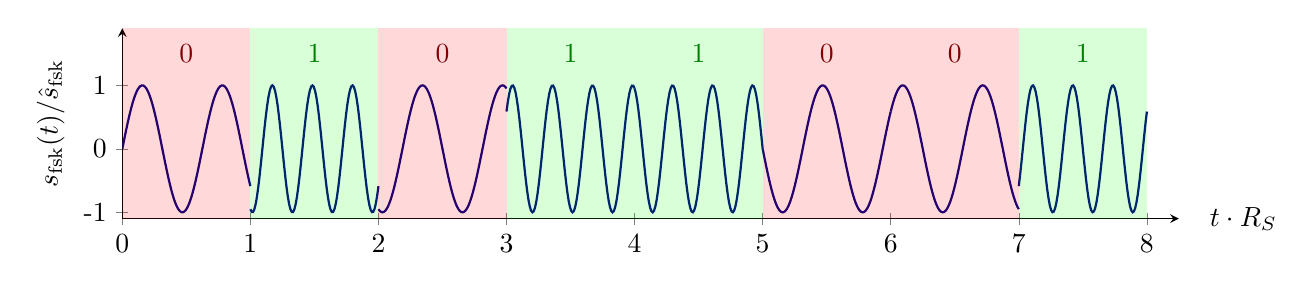
\begin{tikzpicture}
\begin{axis}[
	axis lines = left,
	xlabel = $t \cdot R_S$,
	ylabel = {$s_\mathrm{\gls{fsk}}(t) / \hat s_\mathrm{\gls{fsk}}$},
	yticklabels = {,-1, 0, 1},
	xticklabels = {,0,1,2,3,4,5,6,7,8},
	width = 15cm,
	height = 4cm,
	every axis plot/.append style = {thick},
	%axis x line = center,
	xmax = 6.5,
	ymax = 1.9,
	ymin = -1.1,
	every axis x label/.style = {
		at={(ticklabel* cs:1.02)},
		anchor=west,
	}
]
	\addplot [
		domain = -10:-8,
		samples = 100,
		color = blue!50!black
	] {sin(2 * pi * 0.8 * deg(x))};
	\addplot [
		domain = -8:-6,
		samples = 100,
		color = blue!50!black
	] {-sin(2 * pi * 1.6 * deg(x))};
	\addplot [
		domain = -6:-4,
		samples = 100,
		color = blue!50!black
	] {-sin(2 * pi * 0.8 * deg(x))};
	\addplot [
		domain = -4:-2,
		samples = 100,
		color = blue!50!black
	] {-sin(2 * pi * 1.6 * deg(x))};
	\addplot [
		domain = -2:0,
		samples = 100,
		color = blue!50!black
	] {-sin(2 * pi * 1.6 * deg(x))};
	\addplot [
		domain = 0:2,
		samples = 100,
		color = blue!50!black
	] {-sin(2 * pi * 0.8 * deg(x))};
	\addplot [
		domain = 2:4,
		samples = 100,
		color = blue!50!black
	] {-sin(2 * pi * 0.8 * deg(x))};
	\addplot [
		domain = 4:6,
		samples = 100,
		color = blue!50!black
	] {-sin(2 * pi * 1.6 * deg(x))};

	\fill [fill = red, opacity = 0.15] (axis cs: -10, -1.1) rectangle (axis cs: -8, 2);
	\fill [fill = green, opacity = 0.15] (axis cs: -8, -1.1) rectangle (axis cs: -6, 2);
	\fill [fill = red, opacity = 0.15] (axis cs: -6, -1.1) rectangle (axis cs: -4, 2);
	\fill [fill = green, opacity = 0.15] (axis cs: -4, -1.1) rectangle (axis cs: -2, 2);
	\fill [fill = green, opacity = 0.15] (axis cs: -2, -1.1) rectangle (axis cs: 0, 2);
	\fill [fill = red, opacity = 0.15] (axis cs: 0, -1.1) rectangle (axis cs: 2, 2);
	\fill [fill = red, opacity = 0.15] (axis cs: 2, -1.1) rectangle (axis cs: 4, 2);
	\fill [fill = green, opacity = 0.15] (axis cs: 4, -1.1) rectangle (axis cs: 6, 2);

	\node [color = red!50!black] at (axis cs: -9, 1.5) {0};
	\node [color = green!50!black] at (axis cs: -7, 1.5) {1};
	\node [color = red!50!black] at (axis cs: -5, 1.5) {0};
	\node [color = green!50!black] at (axis cs: -3, 1.5) {1};
	\node [color = green!50!black] at (axis cs: -1, 1.5) {1};
	\node [color = red!50!black] at (axis cs: 1, 1.5) {0};
	\node [color = red!50!black] at (axis cs: 3, 1.5) {0};
	\node [color = green!50!black] at (axis cs: 5, 1.5) {1};
	\end{axis}
\end{tikzpicture}
\caption{\gls{fsk}-modulated passband signal, abrupt phase changes}
\label{fig:fsk_gfsk_fsk}
\end{subfigure}
\begin{subfigure}{\textwidth}
\begin{tikzpicture}
\begin{axis}[
	axis lines = left,
	xlabel = $t \cdot R_S$,
	ylabel = {$s_\mathrm{\gls{gfsk}}(t) / \hat s_\mathrm{\gls{gfsk}}$},
	yticklabels = {,-1, 0, 1},
	xticklabels = {,0,1,2,3,4,5,6,7,8},
	width = 15cm,
	height = 4cm,
	every axis plot/.append style = {thick},
	%axis x line = center,
	xmax = 6.5,
	ymax = 1.9,
	ymin = -1.1,
	every axis x label/.style = {
		at={(ticklabel* cs:1.02)},
		anchor=west,
	}
]

	\addplot [color = blue!50!black] table [mark = none, x = x, y = y, col sep = comma] {fig/gfsk_sample.csv};

	\fill [fill = red, opacity = 0.15] (axis cs: -10, -1.1) rectangle (axis cs: -8, 2);
	\fill [fill = green, opacity = 0.15] (axis cs: -8, -1.1) rectangle (axis cs: -6, 2);
	\fill [fill = red, opacity = 0.15] (axis cs: -6, -1.1) rectangle (axis cs: -4, 2);
	\fill [fill = green, opacity = 0.15] (axis cs: -4, -1.1) rectangle (axis cs: -2, 2);
	\fill [fill = green, opacity = 0.15] (axis cs: -2, -1.1) rectangle (axis cs: 0, 2);
	\fill [fill = red, opacity = 0.15] (axis cs: 0, -1.1) rectangle (axis cs: 2, 2);
	\fill [fill = red, opacity = 0.15] (axis cs: 2, -1.1) rectangle (axis cs: 4, 2);
	\fill [fill = green, opacity = 0.15] (axis cs: 4, -1.1) rectangle (axis cs: 6, 2);

	\node [color = red!50!black] at (axis cs: -9, 1.5) {0};
	\node [color = green!50!black] at (axis cs: -7, 1.5) {1};
	\node [color = red!50!black] at (axis cs: -5, 1.5) {0};
	\node [color = green!50!black] at (axis cs: -3, 1.5) {1};
	\node [color = green!50!black] at (axis cs: -1, 1.5) {1};
	\node [color = red!50!black] at (axis cs: 1, 1.5) {0};
	\node [color = red!50!black] at (axis cs: 3, 1.5) {0};
	\node [color = green!50!black] at (axis cs: 5, 1.5) {1};
	\end{axis}
\end{tikzpicture}
\caption{\gls{gfsk}-modulated passband signal, continuous phase}
\label{fig:fsk_gfsk_gfsk}
\end{subfigure}
\caption{Comparison of \gls{fsk} and \gls{gfsk} for the same binary input sequence. For demonstration purposes, a very low carrier frequency in reference to symbol rate and frequency shift is shown.}
\label{fig:fsk_gfsk_comparison}
\end{figure}


\subsection{Implementation by Sigfox}
Just like uplinks, Sigfox downlinks are transmitted in a license-free band whose frequency range depends on the local regulations of the geographic region.
Under \gls{etsi} regulations in Europe, the assigned frequency range is 869.4 MHz to 869.65 MHz with a maximum transmission power of 500 mW and a $10\%$ duty cycle (see also \Cref{fig:srd_bands}) \cite[Section 5.2.1]{sigfox_ietf}.
The symbol rate is $600 ~ \mathrm{Bd}$ for all regions and since the downlink's modulation scheme is binary \gls{gfsk}, that also implies a bit rate of $600 \mathrm{bit} / \mathrm{s}$.
Unlike the uplink's carrier frequency, the downlink's frequency is not randomly chosen but is a function of the frequency of the uplink that requested the downlink, so that the Sigfox object only needs to listen for downlinks on one specific frequency.
While this fact is publicly acknowledged, details on how the downlink frequency is derived from the uplink frequency have not been disclosed \cite[Section 5.2.1]{sigfox_ietf}.
To find out more about this relationship, the downlink's carrier frequency in reference to the initial uplink's carrier frequency was measured.
This was done in close physical proximity of two different base stations in Germany (see \Cref{fig:basestation_photo}) that were previously localized by measuring downlink signal strengths at various locations.
Some initial uplinks were generated by the \textit{Pycom SiPy} while others were manually composed using the reconstructed uplink protocol and transmitted with a \textit{HackRF One} \gls{sdr}.
The resulting measurements are shown in \Cref{fig:ul_dl_dependency}.
Since measurements were carried out with two different \gls{sdr} devices and throughout multiple days, the error margin is unknown.
Based on these measurements, the following relationship between uplink frequency $f_\text{UL}$ and downlink frequency $f_\text{DL}$ is suggested:

\begin{equation}
\begin{array}{c}
f_\text{DL} = \left( \left( f_\text{UL} + \Delta f - f_\text{lower} \right) ~ \bmod ~ f_\text{bandwidth} \right) + f_\text{lower} \\
\text{with} \\
\begin{alignedat}{2}
	\Delta f &= 1.395 ~ \mathrm{MHz} & & ~~ \ldots \text{frequency offset between downlink and uplink} \\
	f_\text{lower} &\approx 869.425 ~ \mathrm{MHz} & & ~~ \ldots \text{downlink band lower limit} \\
	f_\text{bandwidth} &\approx 0.2 ~ \mathrm{MHz} & & ~~ \ldots \text{downlink band bandwidth}
\end{alignedat}
\end{array}
\end{equation}

\begin{figure}[h]
	\centering
	\begin{tikzpicture}[>=latex]
		\begin{axis}[
			axis lines = left,
			xtick={868.0,868.1,...,868.5},
			ytick={869.4,869.5,...,869.6},
			xlabel={$f_\mathrm{UL} ~ [ \mathrm{MHz} ]$},
			ylabel={$f_\mathrm{DL} ~ [ \mathrm{MHz} ]$},
			xmin=867.95,
			xmax=868.45,
			ymin=869.35,
			ymax=869.65,
			domain=867.95:868.4,
			grid=both,
			grid style={line width=.1pt, draw=gray!10},
			major grid style={line width=.2pt,draw=gray!50},
			minor tick num=5,
			width=10cm,
			height=6cm,
			legend pos=outer north east,
			legend entries={suggested relationship, measured relationship}]

			\addlegendimage{no markers, blue},
			\addlegendimage{mark = *, only marks, red}

			\addplot [color = red, mark = *] table [x = f_ul, y = f_dl, only marks, col sep = comma] {fig/dl_ul_freq.csv};

			\addplot [no markers,
				style=thick,
				color=blue,
				domain=868.0:868.030
			] {x + 1.595};
			\addplot [no markers,
				style=thick,
				color=blue,
				domain=868.030:868.230
			] {x + 1.395};
			\addplot [no markers,
				style=thick,
				color=blue,
				domain=868.230:868.4
			] {x + 1.195};
		\end{axis}
	\end{tikzpicture}

	\caption{Downlink frequency $f_\mathrm{DL}$ as a function of the corresponding uplink frequency $f_\mathrm{UL}$}
	\label{fig:ul_dl_dependency}
\end{figure}

\Cref{fig:ul_dl_dependency} shows that measurement and mathematical relationship line up except for minor outliers which could be explained by measurement errors, e.g. due to inaccuracies in the \gls{sdr} hardware and imperfect methods used to determine the respective carrier frequencies of uplink and downlink.
The precise frequency values are guesses based on the measured uplink-downlink frequency pairs.
Since the \textit{SiPy} only appears to transmit uplinks within the limited frequency range of approximately $868.03 ~ \mathrm{MHz}$ to $868.23 ~ \mathrm{MHz}$, the exact values for $f_\text{lower}$ and $f_\text{bandwidth}$ do not seem to appear in the \textit{SiPy}'s firmware image.

As illustrated in \Cref{fig:listening_window_interval}, Sigfox objects like the \textit{SiPy} listen for downlinks for a duration of approximately 25s starting 20s after the initial transmission of the downlink-requesting uplink has been completed \cite[Section 3.2]{stfirmware} \cite[Figure 1-2]{rs_appnote}.

\begin{figure}
	\centering
	\begin{tikzpicture}[x = 0.25cm, y = 0.25cm, font=\sffamily]
		\node (initial) [fill = blue!50!black, minimum height = 1.2cm, minimum width = 1.12] at (0.56, 0.8cm) {};
		\node (replica1) [fill = blue!50!black, minimum height = 1.2cm, minimum width = 1.12] at (2.18, 0.8cm) {};
		\node [fill = blue!50!black, minimum height = 1.2cm, minimum width = 1.12] at (3.80, 0.8cm) {};

		\node [above = 0.5cm of replica1] {Uplink};

		\node (window) [fill = blue!30!white, minimum height = 1.2cm, minimum width = 6.25cm] at (33.62, 0.8cm) {Downlink Listening Window};

		\draw [thick, -latex] (0, 0) -- (50, 0) node[right = 1] {Time $t$};

		\draw (window.south west) -- (window.north west) -- ($(window.north west) + (0, 0.4cm)$);
		\draw (window.south east) -- (window.north east) -- ($(window.north east) + (0, 0.4cm)$);
		\draw [latex-latex] ($(window.north west) + (0, 0.3cm)$) -- ($(window.north east) + (0, 0.3cm)$) node[midway, above] {25s};

		\draw (initial.south east) -- (initial.north east) -- ($(initial.north east) + (0, 0.4cm)$);
		\draw [latex-latex] ($(initial.north east) + (0, 0.3cm)$) -- ($(window.north west) + (0, 0.3cm)$) node[midway, above] {20s};
	\end{tikzpicture}
	\caption{Duration of downlink listening window and interval between uplink and downlink, drawn to scale for a class A uplink, inspired by \cite[Figure 3]{stfirmware}}
	\label{fig:listening_window_interval}
\end{figure}

\subsection{Open Implementation}
As with the uplink's physical layer, the description of the Open Implementation can be divided into two parts:
First, a script that can demodulate a given I/Q-sample recording of a downlink and transform it into a string of bits and second, another script that can take a string of bits and transmit a \gls{gfsk}-modulated signal with an \gls{sdr}.
For recording signals and transmitting them, the setup used is identical to the one used for uplink recording and transmission as described in \Cref{sec:uplink_phy_reimp}, hence the demodulation script takes an I/Q-sample WAV \gls{if} recording as input.

\paragraph{The demodulation script} takes prerecorded I/Q samples as input, so since real-time capabilities are not demanded, a computationally intensive but easy-to-implement demodulation algorithm based on an $\arctan$ demodulator was chosen.
$\arctan$ demodulators are more commonly used to demodulate \gls{fm} signals in software, but can also be employed as a processing stage in \gls{gfsk} signal demodulation.
Descriptions of $\arctan$ demodulators including a block diagrams and explanations of the underlying mathematics are commonly available \cite{fmdemod_arctan}, so a detailed discussion of this stage is omitted here for the sake of brevity.
\Cref{fig:downlink_spectrogram_baseband} shows input and output signals of this stage:
As input, the $\arctan$ demodulator takes the complete I/Q sample recording (represented by the spectrogram in \Cref{fig:downlink_spectrogram}) and as output, it provides a baseband signal (represented by frequency deviation over time as shown in \Cref{fig:downlink_baseband}).
The function of this processing stage can easily be verified by visual inspection and comparison of the prominent frequencies in the spectrogram with the baseband signal output.
In a next step, a preamble, which is part of the downlink frame as later described in \Cref{sec:downlink_frameformat}, is used to synchronize the demodulation script to the recording's symbol timing.
Then, symbols and thus bits are extracted by sampling baseband values and feeding samples into a hard decision decoder.
In the end, the python script outputs the detected downlink frame (excluding the preamble) in hexadecimal format, which is suitable for further processing with \texttt{renard}.

\begin{figure}[h]
\begin{subfigure}[t]{0.425\textwidth}
	\vskip 0pt
	\centering
	\begin{tikzpicture}
		\begin{axis}[
			tick align=outside,
			tick pos=left,
			xmin=0, xmax=80,
			ymin=-22050, ymax=22039,
			xlabel={$t ~ [\mathrm {ms}]$},
			ylabel={$f ~ [\mathrm{kHz}]$},
			yticklabels={-20,-10,0,10,20},
			ytick={-20000,-10000,0,10000,20000},
			scaled y ticks=false,
			width=7cm,
			height=6.65cm
		]
		\addplot graphics [includegraphics cmd=\pgfimage, xmin=0, xmax=80, ymin=-22050, ymax=22039] {fig/downlink_spectrogram.png};
	\end{axis}
	\end{tikzpicture}

	\vspace{0.1cm}
	\caption{Spectrogram of downlink section, colors correspond to power density on a logarithmic scale}
	\label{fig:downlink_spectrogram}
\end{subfigure}
\hspace{0.03\textwidth}
\begin{subfigure}[t]{0.475\textwidth}
	\vspace{0cm}
	\centering
	\includegraphics[width=\textwidth]{fig/downlink_baseband.pdf}
	\vspace{-0.18cm}
	\caption{Baseband signal of same downlink section signal after \gls{fm} demodulation with $\arctan$ demodulator}
	\label{fig:downlink_baseband}
\end{subfigure}
\caption{Spectrogram and baseband signal for a section of the recorded downlink \gls{gfsk} signal, mixed to \gls{if}}
\label{fig:downlink_spectrogram_baseband}
\end{figure}

\paragraph{Downlink modulation} is implemented by a different python script that takes the raw downlink frame in hexadecimal format as input and generates I/Q samples for transmission with an \gls{sdr} such as the \textit{HackRF One} as output.
The hexadecimal input is first converted to a binary sequence which is then transformed into a baseband signal $m_\text{rect}(t)$ with rectangular pulses.
Subsequently, Gaussian filtering is applied to $m_\text{rect}$, generating the baseband signal $m(t)$ so that modulation produces a \gls{gfsk}, and not just an \gls{fsk}, signal.
The additional steps in the modulation script are based on the known equations for \gls{fm} modulation \cite[Equation (4.3.13) and (4.3.14)]{commsys} that describe how the sinusoidal carrier at frequency $f_c$ is modulated generating the passband signal $u(t)$:
\begin{equation}
	u(t) = A_c \cdot \cos \left ( 2 \pi ~ \left ( f_c \cdot t + f_\Delta \cdot \int_{-\infty}^t m(\tau) ~ \mathrm d\tau \right) \right)
\end{equation}
where $A_c$ is the carrier's amplitude and $f_\Delta$ is the maximum frequency deviation, which is half of the passband signal's bandwidth.
This assumes that $m(\tau)$ is limited to $[-1, 1]$, which can be achieved through normalization.
All theoretical processing steps from binary symbols to passband signal are also summarized in \Cref{fig:downlink_fm_mod}.
For Sigfox, a maximum frequency deviation of approximately $f_\Delta = 0.8 \mathrm{kHz} = 800 \mathrm{Hz}$ was found according to \Cref{fig:downlink_baseband}, even though \cite[Section 5.2.1]{sigfox_ietf} suggests otherwise ($1.5 \mathrm{kHz}$ bandwidth, which would correspond to a maximum frequency deviation of $0.75 \mathrm{kHz} = 750 \mathrm{Hz}$).
In practice, the modulation script does not use time-continuous signals $m_\text{rect}(t)$, $m(t)$ and $u(t)$, but discrete-time versions and integration can be described by summation, but the principle is the same.
Also, the script does not directly modulate a sinusoidal carrier at $f_c$, but one at an intermediate frequency $f_\mathrm{IF} = 2 \cdot f_\Delta$.
The final upconversion to the carrier frequency occurs inside the SDR hardware (e.g. \textit{HackRF One}) at transmission time.

\begin{figure}[h]
	\pgfmathdeclarefunction{gauss}{2}{%
		\pgfmathparse{1/(#2*sqrt(2*pi))*exp(-((x-#1)^2)/(2*#2^2))}%
	}

	\centering
	\begin{tikzpicture}[font=\sffamily]
		\node (pulseshaper) [rectangle, thick, draw = black, minimum width = 1.5cm, minimum height = 1.5cm, label=below:Pulse Shaping] {\begin{tikzpicture}
				\draw [-latex, thick] (-0.7, -0.3) -- (0.7, -0.3);
				\draw [-latex, thick] (0, -0.5) -- (0, 0.5);
				\draw [thick, color=red] (-0.5, -0.3) -- (-0.3, -0.3) -- (-0.3, 0.2) -- (0.3, 0.2) -- (0.3, -0.3) -- (0.5, -0.3);
			\end{tikzpicture}};
		\node (gaussfilter) [right = of pulseshaper, rectangle, thick, draw = black, minimum width = 1.5cm, minimum height = 1.5cm, label=below:Filtering] {\begin{tikzpicture}
				\begin{axis}[axis lines=none, width=3cm, height=3cm, ymax=0.7]
					\addplot[thick, color=red, samples=100, no markers]{gauss(0, 1.0)};
					\draw [-latex, thick] (axis cs: -5, 0) -- (axis cs: 5, 0);
					\draw [-latex, thick] (axis cs: 0, 0) -- (axis cs: 0, 0.6);
				\end{axis}
			\end{tikzpicture}};
		\node (normalizer) [right = of gaussfilter, rectangle, thick, draw = black, minimum width = 1.5cm, minimum height = 1.5cm, label=below:Normalization] {\scalebox{1.4}{$\frac{\cdot}{\left \|\cdot \right \|}$}};
		\node (integrator) [right = of normalizer, rectangle, thick, draw = black, minimum width = 1.5cm, minimum height = 1.5cm, label=below:Integration] {$\scalebox{1.4}{$\int$} \mathrm dt$};
		\node (phasemod) [right = of integrator, rectangle, thick, draw = black, minimum width = 1.5cm, minimum height = 1.5cm, align = center] {Phase\\Modulator};

		\draw [-latex, thick] (pulseshaper) -- (gaussfilter);
		\draw [-latex, thick] (gaussfilter) -- (normalizer);
		\draw [-latex, thick] (normalizer) -- node[above] {$m(t)$} (integrator);
		\draw [-latex, thick] (integrator) -- (phasemod);
		\draw [-latex, thick] ($(pulseshaper.west) + (-1, 0)$) node[above] {$s_k \in \{ \pm 1 \}$} -- (pulseshaper);
		\draw [-latex, thick] ($(phasemod.south) + (0, -1)$) node[below, align = center] {Carrier\\$A_c \cdot \cos \left( 2 \pi f_c \cdot t \right)$} -- (phasemod);
		\draw [-latex, thick] (phasemod) -- ($(phasemod.east) + (1, 0)$) node[above] {$u(t)$};
	\end{tikzpicture}
	\caption{Block diagram of processing steps for \gls{gfsk} modulation assuming binary input data $\in \{0, 1\}$ is already antipodally mapped to symbols $s_k \in \{ \pm 1 \}$}
	\label{fig:downlink_fm_mod}
\end{figure}

\FloatBarrier
\subsection{Result}
The downlink modulation scheme discovered by recording frames verifies Sigfox's claims \cite[Section 5.2.1]{sigfox_ietf} concerning the downlink's physical layer in the \gls{etsi} region except for the maximum frequency deviation which was found to be 800 Hz instead of the stated 750 Hz.
The demodulation script can successfully retrieve binary contents of recorded frames and the \textit{Pycom SiPy} accepts forged downlinks transmitted with a \textit{HackRF One}.

Like \gls{dbpsk}, \gls{fsk} is a very common modulation scheme, with \gls{gfsk} being a somewhat less common special case of that.
It is not entirely clear why Sigfox chose to use completely different physical layer implementations for uplink and downlink, but some speculations based on the advantages and disadvantages of \gls{dbpsk} in comparison to \gls{gfsk} can be made.
A major factor in favor of \gls{gfsk} might be the complexity of \gls{dbpsk} demodulation compared to a \gls{gfsk} demodulator.
Since in the case of downlink transmissions, demodulation has to be implemented on the Sigfox object's side which is typically low-power, having existing, efficient RF hardware is a deciding issue.
In case of uplink transmissions, the complexity involved with decoding \gls{unb} \gls{dbpsk} uplinks (Costas loop, precise estimation of carrier frequency) is less relevant as a more powerful base station provides enough computational resources.
Additionally, the constraints on spectral efficiency of downlink transmissions do not have to be as rigorous, because far less downlinks are to be expected due to the limited maximum number of downlink messages per device and day imposed by Sigfox.
Moreover, restrictions on the power consumption of base stations are naturally far less tight, so that a modulation scheme like \gls{gfsk} which has a higher power consumption compared to the very power-efficient \gls{unb} \gls{dbpsk} can be used.
The higher baud rate might be a result of the requirement for downlinks not to take too much time, since base stations need to adhere to duty cycle limitations.
On the other hand, the reasons for different modulation schemes might also be of historical nature as downlink functionality was initially not supported and only added later during development \cite[Section 2.1]{lpwan_comparison}.

It is also noteworthy that for the \gls{etsi} region, Sigfox chose to use different frequency ranges for uplink and downlink, possibly as an adaptation to existing \gls{etsi} regulations for \glspl{srd} \cite{bnetza_srd}.
As \Cref{fig:srd_bands} shows, Sigfox uses a band with a possible 10\% duty cycle and up to 500mW maximum \gls{erp} for the downlink.
Using this band over the 868.0 MHz to 868.6 MHz band (1\% duty cycle) that is used for the uplink makes sense, as duty cycle regulations apply on a per-device basis:
Given that a single Sigfox base station (which is not excempt from these regulations) hypothetically has to serve hundreds of Sigfox objects, a 1\% duty cycle may not suffice to provide them all with downlinks, so a different band with a 10\% duty cycle is more appropriate.
Moreover, the 869.4 MHz to 869.65 Mhz band allows for a heightened transmit power which base stations can exhaust since they are, as opposed to most Sigfox objects, not constrained by limited battery power.

\FloatBarrier
\section{Frame Structure}
\label{sec:downlink_frameformat}
\subsection{Introduction: MAC, CRC and Error Correction}
\label{sec:downlink_frameformat_introduction}
The concepts behind \glspl{mac} and \glspl{crc} were already briefly introduced before describing the uplink's frame structure, see \Cref{sec:uplink_mac_crc}.

In digital communications, inevitable noisy transmission channels cause symbol errors at the demodulator's output \cite[Section 1.2.4]{ecctechniques}.
While these errors could be prevented by e.g. increasing signal power, that is usually not the most economical method to reliably transmit data.
Despite the additional complexity, \gls{fec} using \glspl{ecc} can greatly increase the reliability of transmission systems while keeping energy consumption low \cite[chapter 1, introduction]{ecctechniques}.
This is done by adding redundancy, that is additional bits that are not part of the transmitted payload, to the frame.
A special kind of \glspl{ecc}, \glspl{bcc}, were already discussed in \Cref{sec:ul_repetitions}.
A more thorough introduction to \gls{ecc} coding including the definition of terms like ``code rate'' is left to literature, e.g. \cite{ecctechniques} and more detailed information on the specific use of \glspl{ecc} in the Sigfox downlink is given in \Cref{sec:downlink_ecc}.
In the following and in accordance with Sigfox's nomenclature \cite{sigfox_ietf, rs_appnote}, ``\gls{ecc}'' is used to denominate the redundancy bits in the frame.

\subsection{Implementation by Sigfox}
The downlink's basic frame structure is shown in \cite[Figure 1-2]{rs_appnote}, but the contents of the individual fields are not explained.
By recording several downlinks with an \gls{sdr} in physical proximity of cell towers equipped with Sigfox base stations, parts of this frame structure could be verified.

A Sigfox downlink consists of only one single frame without any transmission repetitions.
As of May 2018, the downlink frame always contains 8 bytes of data and the Sigfox web interface does not permit entering a different number of bytes, so that the downlink's frame structure is static and much simpler than the uplink's.
The basic structure of a downlink frame is shown in \Cref{fig:downlink_frameformat}.

\begin{figure}[h]
\begin{subfigure}[c]{1.0\textwidth}
	\centering
	\def\dlfbitsize{0.065} % x-size of bit in frame
	\def\lineheight{0.9}

	\begin{tikzpicture}[font=\sffamily]
		% Frame structure
		\draw [fill=black, thick] (0,0) rectangle (104 * \dlfbitsize,\lineheight) node[pos=.5, color=white] {Preamble};
		\draw [thick, pattern = north east lines, pattern color = black!20!white] (104 * \dlfbitsize,0) rectangle (136 * \dlfbitsize,\lineheight) node[pos=.5] {\glsunset{ecc} \gls{ecc} \glsreset{ecc}};
		\draw [thick, pattern = north east lines, pattern color = black!20!white] (136 * \dlfbitsize,0) rectangle (200 * \dlfbitsize,\lineheight) node[pos=.5] {Payload};
		\draw [thick, pattern = north east lines, pattern color = black!20!white] (200 * \dlfbitsize,0) rectangle (216 * \dlfbitsize ,\lineheight) node[pos=.5] {MAC};
		\draw [thick, pattern = north east lines, pattern color = black!20!white] (216 * \dlfbitsize,0) rectangle (224 * \dlfbitsize,\lineheight) node[pos=.5] {C};

		% Frame bit numbers
		\foreach \x in {0, 104, 136, 200, 216} {
			\draw [thick] (\x * \dlfbitsize, \lineheight) -- (\x * \dlfbitsize, \lineheight + 0.1);
			\node [anchor=south] at (\x * \dlfbitsize, \lineheight) {\footnotesize \x};
		}
		\draw [thick] (224 * \dlfbitsize, \lineheight) -- (224 * \dlfbitsize, \lineheight + 0.1);
		\node [anchor=south west] at (224 * \dlfbitsize, \lineheight) {\footnotesize 224};

		% legend
		\node (legend) at (0, -0.2em) [anchor = north west, minimum width = \textwidth] {\begin{tikzpicture}
			\node [minimum width = 0cm] (crclegend) {\sffamily C = \gls{crc}-8};
			\node [right = of crclegend, minimum height = 0.5cm, minimum width = 0.5cm, pattern = north east lines, pattern color = black!20!white] (checkerpattern) {};
			\node [right = 0em of checkerpattern, minimum width = 0cm] (scrambledlegend) {\sffamily = scrambled};
\end{tikzpicture}};
	\end{tikzpicture}
\end{subfigure}
\begin{subfigure}[c]{1.0\textwidth}
	\centering
	\begin{tabular}{r c p{10cm}}
		\textbf{Preamble} & 13 bytes & Predefined pattern for receiver synchronization: \texttt{0x2aaaaaaaaaaaaaaaaaaaaab227} \\
		\textbf{ECC} & 4 bytes & Redundancy information for error correction \\
		\textbf{Payload} & 8 bytes & Message to be transmitted \\
		\textbf{\gls{mac}} & 2 bytes & Message Authentication Code \\
		\textbf{CRC-8} & 1 byte & 8-bit \gls{crc} checksum
	\end{tabular}
\end{subfigure}
\caption{Static downlink frame structure}
\label{fig:downlink_frameformat}
\end{figure}

The frame starts with a 13-byte \textbf{preamble} that contains the constant pattern
\[
	\text{\texttt{0x2aaaaaaaaaaaaaaaaaaaaab227}}
\]
This pattern was found by recording multiple downlinks from the two different base stations shown in \Cref{fig:basestation_photo}.

The other fields of the frame (\gls{ecc}, payload, \gls{mac} tag and \gls{crc}-8) are scrambled, so the contents are not plainly readable.
Since scrambling and descrambling will be explained in \Cref{sec:downlink_scrambling}, the following is written under the assumption that descrambling has already occurred and the frame contents are present as plaintext.

After the preamble 4 bytes for error correction follow, here denominated by ``\textbf{\gls{ecc}}''.
This redundancy information is used to correct errors in payload, \gls{mac} tag and / or \gls{crc}.
More detailed information on the composition of these bytes and on the types of \glspl{ecc} used will be given in \Cref{sec:downlink_ecc}.

The \gls{ecc} field is followed by the 8-byte \textbf{payload}.
The length of the payload is static, so if a user wishes to transmit less than 8 bytes, the remaining bits have to be padded with some data.
As with the uplink frame, the payload is not encrypted in any way, but as previously stated, along with the \gls{ecc}, \gls{mac} tag and \gls{crc} fields it is scrambled as described in \Cref{sec:downlink_scrambling}.

The subsequent field is the \textbf{\gls{mac}} tag which, in contrast to the uplink's \gls{mac} tag, has a constant length of 2 bytes.
The \gls{mac} protects the integrity of the payload against malicious modification after \gls{fec} with the \gls{ecc} information has been applied.
It does not protect the integrity of preamble or \gls{crc}.
The computation of the \gls{mac} tag will be detailed in \Cref{sec:downlink_mac}.

The final downlink field is the \textbf{\gls{crc}} checksum.
Contrary to the uplink which uses a 16-bit checksum, the downlink uses a \gls{crc}-8 which requires only 8 bits.
The \gls{ecc} data supplied with the downlink frame can be used to correct a limited number of bit errors, so the \gls{crc}-8 only needs to protect the integrity of payload and \gls{mac} tag fields against bit errors if more bit errors occur than can be corrected or if the frame is not actually a Sigfox downlink destined for the object that received it.

It is noteworthy that the downlink frame does not contain any device ID or \gls{sn}.
A different mechanism that involves the scrambler using different \glspl{prbs}, depending on device ID and \gls{sn} of the foregone uplink is used instead.
The details of scrambling will be described in \Cref{sec:downlink_scrambling}, but, in summary, this method results in devices without matching device ID or \gls{sn} to produce a garbled bit stream after the descrambler, which causes both \gls{crc} and \gls{mac} tag checks to fail with a high probability.

\subsection{Open Implementation}
Downlink encoding is also implemented in \texttt{librenard}, access via a command line interface is provided by \texttt{renard}.
The steps required for downlink frame construction are summarized in \Cref{fig:downlink_encoding}, which also shows that for constructing a valid downlink, not only payload but also the Sigfox object's \gls{nak} and device ID as well as the \gls{sn} of the uplink that requested the downlink are necessary.

\begin{figure}[h]
	\centering
	\scalebox{0.8}{\begin{tikzpicture}
			% steps
			\node at (0, 0) [align = center, rectangle, minimum height = 2em, minimum width = 10em, rounded corners = 4] (entry) {};
			\node [align = center, draw, rectangle, minimum height = 2em, minimum width = 10em, rounded corners = 4, below = 1em of entry] (mactag) {Compute \gls{mac} tag};
			\node [align = center, draw, rectangle, minimum height = 2em, minimum width = 10em, rounded corners = 4, below = 1em of mactag] (crc) {Compute \gls{crc}};
			\node [align = center, draw, rectangle, minimum height = 2em, minimum width = 10em, rounded corners = 4, below = 1em of crc] (ecc) {Add \gls{ecc}};
			\node [align = center, draw, rectangle, minimum height = 2em, minimum width = 10em, rounded corners = 4, below = 1em of ecc] (scramble) {Scramble};
			\node [align = center, draw, rectangle, minimum height = 2em, minimum width = 10em, rounded corners = 4, below = 1em of scramble] (preamble) {Add preamble};

			% arrows between steps
			\draw [-latex] (mactag) -- (crc);
			\draw [-latex] (crc) -- (ecc);
			\draw [-latex] (ecc) -- (scramble);
			\draw [-latex] (scramble) -- (preamble);

			% frames at various steps
			\node [draw, thick, rectangle, right = 2em of entry, minimum width = 12em, minimum height = 1.8em] (payload_plain) {\sffamily Payload};

			\node [draw, thick, rectangle, right = 2em of mactag, minimum width = 12em, minimum height = 1.8em] {\sffamily Payload};
			\node [draw, thick, rectangle, right = 14em of mactag, minimum width = 3em, minimum height = 1.8em] (mac_mac) {\sffamily \gls{mac}};

			\node [draw, thick, rectangle, right = 2em of crc, minimum width = 12em, minimum height = 1.8em] (payload_crc) {\sffamily Payload};
			\node [draw, thick, rectangle, right = 14em of crc, minimum width = 3em, minimum height = 1.8em] {\sffamily \gls{mac}};
			\node [draw, thick, rectangle, right = 17em of crc, minimum width = 1.5em, minimum height = 1.8em] (crc_crc) (crc_crc) {\sffamily C};

			\node [draw, thick, rectangle, right = 2em of ecc, minimum width = 6em, minimum height = 1.8em] {\sffamily \gls{ecc}};
			\node [draw, thick, rectangle, right = 8em of ecc, minimum width = 12em, minimum height = 1.8em] (payload_ecc) {\sffamily Payload};
			\node [draw, thick, rectangle, right = 20em of ecc, minimum width = 3em, minimum height = 1.8em] {\sffamily \gls{mac}};
			\node [draw, thick, rectangle, right = 23em of ecc, minimum width = 1.5em, minimum height = 1.8em] (crc_ecc) {\sffamily C};

			\draw (crc_crc.south east) -- (crc_ecc.north east);
			\draw (payload_crc.south west) -- (payload_ecc.north west);

			\node [draw, pattern = north east lines, pattern color = black!20!white, thick, rectangle, right = 2em of scramble, minimum width = 6em, minimum height = 1.8em] (ecc_scrambled) {\sffamily \gls{ecc}};
			\node [draw, pattern = north east lines, pattern color = black!20!white, thick, rectangle, right = 8em of scramble, minimum width = 12em, minimum height = 1.8em] {\sffamily Payload};
			\node [draw, pattern = north east lines, pattern color = black!20!white, thick, rectangle, right = 20em of scramble, minimum width = 3em, minimum height = 1.8em] {\sffamily \gls{mac}};
			\node [draw, pattern = north east lines, pattern color = black!20!white, thick, rectangle, right = 23em of scramble, minimum width = 1.5em, minimum height = 1.8em] (crc_scrambled) {\sffamily C};

			\node [draw, fill = black, text = white, thick, rectangle, right = 2em of preamble, minimum width = 9.75em, minimum height = 1.8em] {\sffamily Preamble};
			\node [draw, pattern = north east lines, pattern color = black!20!white, thick, rectangle, right = 11.75em of preamble, minimum width = 11.25em, minimum height = 1.8em] (combined) {\footnotesize \sffamily \gls{ecc}, Payload, \gls{mac}, \gls{crc}-8};

			\draw (ecc_scrambled.south west) -- (combined.north west);
			\draw (crc_scrambled.south east) -- (combined.north east);

			% input data
			\draw [-latex] ($(payload_plain.west) + (-13em, 0)$) node [anchor = east] {\sffamily Payload} -- (payload_plain.west);
			\draw [-latex] ($(mactag.west) + (-1em, 0)$) node [anchor = east] {\sffamily \gls{nak}} -- (mactag.west);
			\draw [-latex] ($(scramble.west) + (-1em, 0)$) node [anchor = east, align = center] {\sffamily Device ID, \gls{sn}} -- (scramble.west);

			% steps background
			\draw [rounded corners = 5, dashed, very thick, color = black!20!white] ($(mactag.north west) + (-0.4em, 0.4em)$) rectangle ($(mac_mac.south east) + (0.4em, -0.4em)$);
			\draw [rounded corners = 5, dashed, very thick, color = black!20!white] ($(crc.north west) + (-0.4em, 0.4em)$) rectangle ($(crc_crc.south east) + (0.4em, -0.4em)$);
			\draw [rounded corners = 5, dashed, very thick, color = black!20!white] ($(ecc.north west) + (-0.4em, 0.4em)$) rectangle ($(crc_ecc.south east) + (0.4em, -0.4em)$);
			\draw [rounded corners = 5, dashed, very thick, color = black!20!white] ($(scramble.north west) + (-0.4em, 0.4em)$) rectangle ($(crc_scrambled.south east) + (0.4em, -0.4em)$);
			\draw [rounded corners = 5, dashed, very thick, color = black!20!white] ($(preamble.north west) + (-0.4em, 0.4em)$) rectangle ($(combined.south east) + (0.4em, -0.4em)$);

			% legend
			\node (legend) [below = 1em of preamble.south west, anchor = north west, minimum width = \textwidth] {\begin{tikzpicture}
				\node [minimum width = 0cm] (crclegend) {\sffamily C = \gls{crc}-8};
				\node [right = of crclegend, minimum height = 0.5cm, minimum width = 0.5cm, pattern = north east lines, pattern color = black!20!white] (checkerpattern) {};
				\node [right = 0em of checkerpattern, minimum width = 0cm] (scrambledlegend) {\sffamily = scrambled};
\end{tikzpicture}};

	\end{tikzpicture}}
	\caption{Downlink frame construction by \texttt{librenard} including frame contents after each processing step and required input data}
	\label{fig:downlink_encoding}
\end{figure}


\texttt{librenard} also implements decoding of downlinks, including \gls{fec} with the \gls{ecc} data and checking \gls{mac} tag and \gls{crc}.
Obtaining the payload from a recorded Sigfox downlink with \texttt{librenard}'s command line interface, \texttt{renard}, is possible if either
\begin{enumerate}
\item the downlink frame, the object's device ID and the \gls{sn} of the uplink frame that requested the downlink are known
\item the downlink frame, the object's device ID and \gls{nak} are known
\item the downlink frame is known and the signal does not contain any bit errors that have to be corrected by \gls{fec}
\end{enumerate}
The reasons for this are detailed in \Cref{sec:downlink_scrambling_reimp}.

\subsection{Result}
The downlink's frame structure that was reconstructed is much simpler than the uplink's structure, but remarkably uses scrambling and contains \gls{fec} information.
The supposed frame structure was verified by comparing manually generated frames with ones that were generated by base stations and by sending forged downlinks to a Sigfox object (\textit{Pycom SiPy}).

Interestingly, the \textit{Pycom SiPy}, and so presumably other Sigfox objects as well, do not need to receive the entire preamble pattern to synchronize their receiver clocks, the final four bytes \texttt{0xaaaab227} suffice.
This was tested by sending forged downlink frames with shortened preambles, e.g. with an \gls{sdr} such as the \textit{HackRF One}.

It has also been verified that the \textit{Pycom SiPy} actually implements \gls{fec}. The code rate of the \gls{fec} was found to be $\frac{11}{15}$, a rate in this range is not uncommon for wireless communication systems.

\FloatBarrier
\section{Authentication Tag Generation}
\label{sec:downlink_mac}
\subsection{Introduction: Authentication and CBC-MAC}
The basic purpose of \glspl{mac} has already been introduced in \Cref{sec:uplink_mac_crc} and \glspl{cbcmac} have been described in greater detail in \Cref{sec:uplink_mac_introduction}.
No further introduction is required to understand the authentication mechanisms defined in the downlink protocol.

\subsection{Implementation by Sigfox}
The downlink uses the same \gls{aes}-128-based \gls{cbcmac} algorithm as the uplink, even the encryption key is the same shared \gls{nak} that is also used for generating the uplink's \gls{mac} tag.
The differences between uplink and downlink lie in the different plaintext that is input to the \gls{cbcmac} algorithm as well as the length of the \gls{mac} tag.

\Cref{fig:downlink_macinput_composition} shows the content of the 128-bit constant-length plaintext message that is provided as input to the \gls{aes}-128-\gls{cbc} algorithm (in this case, the use of \gls{cbc} mode is irrelevant since the plaintext consists of a single 128-bit block anyway).
Remarkably and contrary to the uplink's \gls{mac}, the downlink's \gls{mac} tag not only depends on the frame contents (which would be only the payload in this case), but also on device ID and the \gls{sn} of the requesting uplink.
The device ID is stored in little-endian format (as with the uplink), the 12-bit uplink \gls{sn} is prepended with four zeroes and also stored in little-endian format (contrary to the uplink).

The total length of device ID, \gls{sn} with prepended zeroes and payload is $4 + 2 + 8 = 14$ bytes, which means that 2 more bytes are missing in the 16-byte \gls{aes}-128 plaintext block.
Therefore, the plaintext block always has to be padded with a constant number of 2 more bytes.
Again, the ``wrap padding'' method described in \Cref{sec:ul_mac_realization} is used to pad the complete plaintext block:
In case of the downlink, repeating the first 2 bytes of the plaintext block means that the two \glspl{msb} of the device ID are copied.

Unlike the uplink's, the downlink's \gls{mac} tag has a constant length:
The first 2 bytes of the ciphertext that resulted out of the \gls{aes}-128 encryption are used as \gls{mac} tag.

\begin{figure}[h]
	\centering

	\begin{tikzpicture}
		\def\bitsize{0.11cm} % x-size of bit in packet
		\def\lineheight{0.8}
		\def\macalgoffsety{-2}

		% Input format
		\draw [line width = 0.5mm] (0, -\lineheight) rectangle (128 * \bitsize, 0);
		\draw [thick] (0, -\lineheight) rectangle (32 * \bitsize, 0) node[pos=.5] {\sffamily Device ID};
		\draw [thick] (32 * \bitsize, -\lineheight) rectangle (48 * \bitsize, 0) node[pos=.5] {\sffamily \texttt{0000\gls{sn}}};
		\draw [thick] (48 * \bitsize, -\lineheight) rectangle (112 * \bitsize, 0) node[pos=.5] {\sffamily Payload};
		\draw [thick] (112 * \bitsize, -\lineheight) rectangle (128 * \bitsize, 0) node[pos=.5] {\sffamily ID[0:1]};

		% Input bit numbers
		\foreach \x in {0, 32, 48, 112, 128} {
			\draw [thick] (\x * \bitsize, 0) -- (\x * \bitsize, 0.1);
			\node [anchor=south] at (\x * \bitsize, 0) {\sffamily \x};
		}

		% AES function
		\node [rectangle, draw, rounded corners = 3pt, fill = black!10!white, minimum width = 4cm, minimum height = 1cm] (macfunction) at (90 * \bitsize, \macalgoffsety) {\textbf{\texttt{AES-128-CBC}}};
		\draw [thick, -latex] (90 * \bitsize, -\lineheight) -- (macfunction.north);

		\node (nak) [right = 0.5cm of macfunction] {Key (\gls{nak})};
		\draw [thick, -latex] (nak) -- (macfunction);

		% Tag output
		\node [anchor = north, minimum width = 2.1cm, minimum height = 0.25cm, fill=black!20!white] (macinctx) at ($(macfunction.south) + (0, -0.5cm)$) {};
		\node [anchor = north, minimum width = 2cm, minimum height = 2cm, draw, thick] (ctx) at ($(macfunction.south) + (0, -0.5cm)$) {Ciphertext};
		\node [anchor = west] (mac) at ($(macinctx.east) + (1cm, 0)$) {\gls{mac} Tag};
		\draw [thick, -latex] (macfunction.south) -- (ctx.north);
		\draw [thick, -latex] (macinctx.east) -- (mac.west);

		% Legend
		\node [anchor = north west] at (-0.3cm, -1cm) {\begin{tikzpicture}
			\node [anchor = north west] at (0, -0.15cm) {$\bullet$ \texttt{0000\gls{sn}} = \gls{sn} with \texttt{0b0000} prepended};
			\node [anchor = north west] at (0, -0.6cm) {$\bullet$ ID[0:1] = 1\textsuperscript{st} and 2\textsuperscript{nd} \glspl{msb} of device ID};
			\node [anchor = north west] at (0, -1.2cm) {$\bullet$ Device ID, \texttt{0000\gls{sn}}, ID[0:1]: little-endian};
		\end{tikzpicture}};
	\end{tikzpicture}
	\caption{Composition of the plaintext message that the \gls{mac} tag authenticates in the case of a Sigfox downlink}
	\label{fig:downlink_macinput_composition}
\end{figure}

\subsection{Open Implementation}
\texttt{librenard} uses the same \gls{aes}-128 implementation by Texas Instruments \cite{tiaes} for generating the downlink's \gls{mac} tag as for the uplink (see \Cref{sec:uplink_mac_reimp}).
\texttt{librenard} can both generate and validate downlink \gls{mac} tags, albeit obviously only if the \gls{nak} of the target Sigfox object is known.
Apart from the downlink's payload, \texttt{renard} also requires device ID, \gls{sn} and \gls{nak} as parameters when encoding a downlink frame so that a \gls{mac} tag can be computed.

\subsection{Result}
For equal parameters (payload, \gls{sn}, target object) \texttt{librenard} produces valid \gls{mac} tags that coincide with \gls{mac} tags generated by the Sigfox network.
\texttt{librenard} can also produce \gls{mac} tags for downlink frames with arbitrary payload contents that are accepted by the Sigfox object targeted by the downlink frame.
This leads to the assumption that the specifications for downlink authentication have been entirely understood.
Tests with the \textit{Pycom SiPy} have shown that this specific Sigfox object actually validates the downlink's \gls{mac}.

As previously described for uplink authentication (\Cref{sec:uplink_mac_result}), it seems odd that the protocol designers chose to include the device ID in the plaintext the \gls{mac} is computed for since \glspl{nak} should be unique anyway, thus already producing different \gls{mac} tags for different target objects.
On the other hand, it makes sense to have the \gls{sn} be part of the plaintext string for protection against replay attacks.
If the \gls{mac} did not depend on the \gls{sn} of the corresponding uplink and an adversary were to record a downlink for one specific payload, they could replay this downlink and the target object would accept it in response to any downlink request.
This way, the \gls{mac}'s dependence on the \gls{sn} makes sure the \gls{mac} tag is only valid once for a specific downlink.

The remarks on the security of shortening a \gls{mac} made in \Cref{sec:uplink_mac_result} also apply to the downlink.

\FloatBarrier
\section{CRC Computation}
\subsection{Introduction: CRC}
The purpose of \gls{crc} checksums has been briefly outlined in \Cref{sec:uplink_mac_crc}.
An introduction to the mathematics involved with \gls{crc} computation including the importance of the generator polynomial has been given in \Cref{sec:uplink_crc_introduction}.
Further introductory explanations are not required to understand \gls{crc} computation in the downlink protocol.

\subsection{Implementation by Sigfox}
In contrast to uplink frames that contain 16-bit \glspl{crc}, checksums for downlink frames are only 8 bits long.
This led to the assumption that the downlink uses a \gls{crc}-8 algorithm.
Again, through finding the right set of parameters to the \gls{crc} algorithm and testing these parameters for various recorded downlinks, a matching generator polynomial could be found:
\begin{equation}
	G(X) = X^8 + X^5 + X^3 + X^2 + X + 1
\end{equation}

The hexadecimal representation of this polynomial is \texttt{0x2f}.
Like the uplink's \gls{crc}, the downlink's \gls{crc} can be calculated according to \Cref{eq:crc_basic_equation} presented in the introduction to \gls{crc} arithmetic (\Cref{sec:uplink_crc_introduction}).

The make-up of the message polynomial $M(X)$ is depicted in \Cref{fig:downlink_crc_computation}:
The \gls{crc} checksum only depends on the constant-size contents of downlink payload and \gls{mac} tag.

\begin{figure}[h]
	\centering

	\begin{tikzpicture}[font=\sffamily]
		\def\pbitsize{0.1} % x-size of bit in packet
		\def\lineheight{0.8}
		\def\pktoffsety{0}
		\def\algoffsety{-2}

		\definecolor{packetcolor}{rgb}{0.9,1.0,0.8}
		\definecolor{flagscolor}{rgb}{0.8,0.9,1.0}

		% Input data format
		\draw [line width = 0.5mm] (0, -\lineheight) rectangle (80 * \pbitsize, 0);
		\draw [thick] (0, \pktoffsety - \lineheight) rectangle (64 * \pbitsize, \pktoffsety) node[pos=.5] {Payload};
		\draw [thick] (64 * \pbitsize, \pktoffsety - \lineheight) rectangle (80 * \pbitsize, \pktoffsety) node[pos=.5] {\gls{mac}};

		% Packet bit numbers
		\foreach \x in {0, 64, 80} {
			\draw [thick] (\x * \pbitsize, \pktoffsety) -- (\x * \pbitsize, \pktoffsety + 0.1);
			\node [anchor=south] at (\x * \pbitsize, \pktoffsety) {\x};
		}

		% Message m braces
		\draw [thick, decoration = {brace, raise = 5pt}, decorate] (80 * \pbitsize, \pktoffsety) -- node[align = center, right = 7pt, font=\fontsize{10pt}{10pt}\selectfont] {interpreted as\\polynomial $M(X)$} (80 * \pbitsize, \pktoffsety - \lineheight);

		% CRC function
		\node [rectangle, rounded corners = 3pt, fill = black!10!white, draw, thick, minimum width = 4cm, minimum height = 1.1cm] (crcfunction) at (30 * \pbitsize, \algoffsety) {\textbf{\texttt{\gls{crc}-8 ({\normalfont \ttfamily 0x2f})}}};
		\draw [thick, -latex] (30 * \pbitsize, \pktoffsety - \lineheight) -- (crcfunction.north);

		% crc output
		\node (tag) [right = 1cm of crcfunction] {\gls{crc} checksum};
		\draw [thick, -latex] (crcfunction.east) -- (tag.west);
	\end{tikzpicture}
	\caption{Computation of the \gls{crc}-8 checksum depending on payload and \gls{mac} tag for a downlink packet}
	\label{fig:downlink_crc_computation}
\end{figure}


\subsection{Open Implementation}
A \gls{crc}-8 implementation based on an 8-bit shift register was chosen for \texttt{librenard} due to its simplicity and low memory consumption compared to table-based implementations, which is especially important for embedding in low-memory microcontrollers.
\texttt{librenard} can both compute valid \gls{crc} checksums for forged downlink frames as well as check \glspl{crc} of recorded downlinks.

\subsection{Result}
The \glspl{crc} generated by \texttt{librenard} are accepted by the tested Sigfox object, the \textit{Pycom SiPy}, which actually validates the \gls{crc} checksum and rejects packets with invalid checksums.
The \glspl{crc} of recorded downlink frames are also identical with the ones generated by \texttt{librenard} for the same input parameters.

It makes sense for the \gls{crc}'s value to be a function of payload and \gls{mac} tag and not to depend on the preamble or \gls{ecc} information.
To the contrary, the contents of the \gls{ecc} field depend on the \gls{crc} contents.
Consequently, when decoding a downlink frame, \gls{fec} based on the \gls{ecc} bits can be applied in a first step followed by checking the \gls{crc}-8 value.
By checking the \gls{crc} only after \gls{fec}, bit errors in either payload, \gls{mac} or \gls{crc} can be detected and corrected and a valid \gls{crc} indicates that error correction was successful.

The choice of the uncommon \gls{crc} polynomial, which is sometimes also known as ``CRC-8-AUTOSAR'' \cite[written in Koopman notation ``\texttt{0x97}'']{crc8zoo}, is a bit startling.
Nevertheless, \texttt{0x2f} is a good choice for a \gls{crc}-8 polynomial in the case of Sigfox, since it can reliably detect up to 3 bit errors for a data length of up to 119 bits (the \gls{crc} input data for the Sigfox downlink consists of only 80 bits) \cite[again written in Koopman notation ``\texttt{0x97}'']{crc8_polynomial}.
However, according to \cite{crc8zoo}, other polynomials that appear to be more common, such as \texttt{0x07} (recommended by the former \gls{ccitt}), display similar (but not better) performance for a constant input length of 80 bits.

\FloatBarrier
\section{Error Control Coding}
\label{sec:downlink_ecc}
\subsection{Introduction: Linear Codes, BCH Codes and Interleaving}
\label{sec:downlink_ecc_intro}
\subsubsection{Linear Codes and Syndrome Decoding}
A short introduction on the basic purpose of \glspl{ecc} has already been given in \Cref{sec:downlink_frameformat_introduction}.
Here, a more detailed introduction to the encoding and decoding of linear block code shall be given.

Binary block codes add redundancy to a transmission system by assigning a longer binary sequence of length $n$ (called code word) to every binary message sequence of length $k < n$ and transmitting the code word instead of the raw message.
More formally, an $(n, k)$ block code is a collection of $2^k$ unique code words of length $n$, for each of the $2^k$ possible messages of length $k$ \cite[Section 13.2]{commsys}.
The formal definition of a subset of block codes called ``linear block codes'' and their properties are left to literature such as \cite[Section 13.2]{carlson_commsys}, but some of their most important attributes relevant to this work will be summarized in the following:

Binary linear block codes can be represented by a so-called ``generator matrix'' $\mathbf G ~ \in ~ \{ 0, 1 \}^{k \times n}$ so that every message vector $\mathbf m = (M_1 ~~ M_2 ~ \dots ~ M_k) ~ \in ~ \{ 0, 1 \}^{1 \times k}$ can be unambiguously assigned to a code word vector $\mathbf x = (X_1 ~~ X_2 ~ \dots ~ X_n) ~ \in ~ \{ 0, 1 \}^{1 \times n}$ \cite[Section 13.2]{carlson_commsys}.
This way, the process of \textbf{encoding} a message $\mathbf m$ to obtain a code word $\mathbf x$ can be expressed as
\begin{equation}
	\mathbf x = \mathbf m ~ \mathbf G \qquad \text{(under $\GF(2)$-arithmetic)}
	\label{eq:downlink_generator_encoding}
\end{equation}

So-called ``systematic'' linear block codes are block codes whose code word vectors contain the message vector.
Their generator matrix can be written as
\begin{equation}
	\mathbf G = \left[ \mathbf I^k ~ | ~ \mathbf P \right]
\end{equation}
with $\mathbf I^k$ being the $k \times k$ identity matrix and $\mathbf P ~ \in ~ \{ 0, 1 \} ^ {k \times (n - k)}$.
Every linear block code can be converted into an equivalent systematic code with a generator matrix in the above form \cite[Section 3.4]{ecctechniques}.

\textbf{Decoding} and error correction with systematic linear block codes can be accomplished with a so-called ``parity-check matrix'' and a ``syndrome lookup table''.
The parity check matrix $\mathbf H \in \{ 0, 1 \}^{(n - k) \times n}$ of a systematic $(n, k)$ code is given by \cite[Equation (13.2.14)]{commsys}:
\begin{equation}
	\mathbf H = \left[ \mathbf P^T ~ | ~ \mathbf I^{n - k} \right]
\end{equation}

The so-called syndrome $\mathbf s \in \{ 0, 1 \}^{1 \times (n - k)}$ of a code word $\mathbf {\hat x}$ that was received for a transmitted code word $\mathbf x$ is defined by \cite[Section 13.2, Equation 10]{carlson_commsys}
\begin{equation}
	\mathbf s = (S_1 ~~ S_2 ~ \dots ~ S_{n-k}) = \hat{\mathbf x} ~ \mathbf H^T \qquad \text{(under $\GF(2)$-arithmetic)}
\end{equation}
If a received code word $\hat{\mathbf x}$ is valid, the corresponding syndrome is zero ($\mathbf s = \mathbf 0$).
This can either mean that there were no transmission errors ($\hat{\mathbf x} = \mathbf x$) or there were bit errors ($\hat{\mathbf x} \neq \mathbf x$), but there were so many of them that $\hat{\mathbf x}$ equals some other valid code word \cite[Section 13.2, Syndrome Decoding]{carlson_commsys}.

It is most likely that either the transmission didn't cause any bit errors ($\hat{\mathbf x} = \mathbf x$) or that one of the bit patterns $\hat{\mathbf x}$ with the fewest number of errors was received.
In that case, if $\mathbf s \neq \mathbf 0$, the syndrome can be used to find the positions of erroneous bits in the received code word $\hat{\mathbf x}$.
This can be done by generating a so-called ``syndrome lookup table'', that assigns an error vector $\mathbf e$ to every one of the $2^{n - k}$ possible syndromes \cite[Section 13.2, Syndrome Decoding]{carlson_commsys}.
If all possible syndromes are denoted by $\mathbf s^{(0)} = \mathbf 0$, $\mathbf s^{(1)}$, \ldots, $\mathbf s^{\left(2^{n - k} - 1 \right)}$ and all error vectors are denoted by $\mathbf e^{(0)} = \mathbf 0$, $\mathbf e^{(1)}$, \ldots, $\mathbf e^{\left(2^{n - k} - 1 \right)}$ the syndrome lookup table can be written as:
\begin{center}
\begin{tabular}{| c | c |}
	\hline \textbf{Syndrome} & \textbf{Error Vector} \\ \hline \rule{0pt}{2.6ex}
	$\mathbf s^{(0)} = \mathbf 0$ & $\mathbf e^{(0)} = \mathbf 0$ \\
	$\mathbf s^{(1)}$ & $\mathbf e^{(1)}$ \\
	$\mathbf s^{(2)}$ & $\mathbf e^{(2)}$ \\
	\vdots & \vdots \\
	$\mathbf s^{\left(2^{n - k} - 1 \right)}$ & $\mathbf e^{\left(2^{n - k} - 1 \right)}$ \\ \hline
\end{tabular}
\end{center}

Finally, the bit errors can be corrected by combining the received code word $\hat{\mathbf x}$ with the error vector $\mathbf e$ in an XOR operation, forming a valid, error-corrected code word $\mathbf y$:
\begin{equation}
	\mathbf y = \hat{\mathbf x} ~ \oplus ~ \mathbf e
\end{equation}

If the code is systematic and error correction was successful, $\mathbf y$ contains the transmitted message vector $\mathbf m$.

\subsubsection{BCH codes}
Cyclic codes are a subset of linear block codes and \glspl{bchcode} are a subset of cyclic codes.
Definitions for cyclic codes and \glspl{bchcode} would be outside the scope of this work and are left to literature, e.g. \cite[chapter 4]{ecctechniques}.
It is important to note that both cyclic codes and \glspl{bchcode} can also be expressed by a generator matrix $\mathbf G$.
Different \glspl{bchcode} are usually labeled with a 3-tuple $(n, k, t)$ where $n$ stands for the length of code words, $k$ represents the length of message sequences and $t$ is the number of erroneous bits the specific \gls{bchcode} can correct.

\subsubsection{Interleaving}
In practice, communication channels are often influenced by physical effects like fading or crosstalk.
Because of this, bit errors occur in so-called bursts, so that if the $k$\textsuperscript{th} bit of a transmission is erroneous, it is likely that the error spans several successive bits so that the $(k + 1)$\textsuperscript{th} bit is flipped as well.
These conditions are unfavorable for block codes:
For instance, assume a block code that can correct single-bit errors and a transmission protocol in which one complete code word of the block code is transmitted after the next.
If then two adjacent bits of a transmitted frame are flipped while the rest of the frame is correct, both bits likely belong to the same code word and the receiver thus cannot correct the two transmission errors.

Knowing that bit errors often occur in direct succession, one can design a coding scheme so that even adjacent bit errors can be combatted by ``spreading out'' code words across the whole frame.
This is known as \textbf{interleaving} and is best described by \Cref{fig:downlink_interleaving_demo}.
In the upper bit stream, the code words $\mathbf x = (X_1 ~~ X_2 ~~ X_3)$, $\mathbf y = (Y_1 ~~ Y_2 ~~ Y_3)$ and $\mathbf z = (Z_1 ~~ Z_2 ~~ Z_3)$ are transmitted coherently, one after the other.
The interleaver at the sender intertwines code words by taking turns at transmitting the first bit of the first code word $X_0$, then the first bit of the second code word $Y_0$, then the first bit of the third code word $Z_0$, then the second bit of the first code word $X_1$ and so on.
This process is reversed by the deinterleaver at the receiver.

\begin{figure}[h]
	\centering
	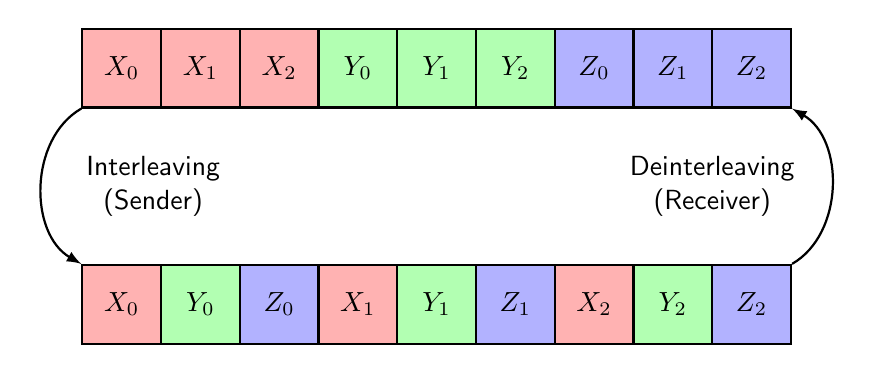
\begin{tikzpicture}[font=\sffamily]
		\def\interleavedy{-3cm}

		\foreach \x in {0, 1, 2} {
			\node (x\x) [draw, thick, minimum width = 1cm, minimum height = 1cm, color = black, fill = red!30!white] at (\x * 1cm, 0) {$X_\x$};
		}
		\foreach \x in {0, 1, 2} {
			\node (y\x) [draw, thick, minimum width = 1cm, minimum height = 1cm, color = black, fill = green!30!white] at (\x * 1cm + 3cm, 0) {$Y_\x$};
		}
		\foreach \x in {0, 1, 2} {
			\node (z\x) [draw, thick, minimum width = 1cm, minimum height = 1cm, color = black, fill = blue!30!white] at (\x * 1cm + 6cm, 0) {$Z_\x$};
		}

		\foreach \x in {0, 1, 2} {
			\node (interx\x) [draw, thick, minimum width = 1cm, minimum height = 1cm, color = black, fill = red!30!white] at (\x * 3cm, \interleavedy) {$X_\x$};
		}
		\foreach \x in {0, 1, 2} {
			\node (intery\x) [draw, thick, minimum width = 1cm, minimum height = 1cm, color = black, fill = green!30!white] at (\x * 3cm + 1cm, \interleavedy) {$Y_\x$};
		}
		\foreach \x in {0, 1, 2} {
			\node (interz\x) [draw, thick, minimum width = 1cm, minimum height = 1cm, color = black, fill = blue!30!white] at (\x * 3cm + 2cm, \interleavedy) {$Z_\x$};
		}

		\draw [thick, -latex] (x0.south west) to [out = 210, in = 150] (interx0.north west);
		\draw [thick, latex-] (z2.south east) to [out = 330, in = 30] (interz2.north east);
		\node [color = black, align = center] at (0.4cm, \interleavedy * 0.5) {Interleaving\\(Sender)};
		\node [color = black, align = center] at (7.5cm, \interleavedy * 0.5) {Deinterleaving\\(Receiver)};
	\end{tikzpicture}
	\caption{Illustration of interleaving and deinterleaving for an unrealistically small code word length of 3 bits}
	\label{fig:downlink_interleaving_demo}
\end{figure}

\subsection{Implementation by Sigfox}
\subsubsection{Interleaving and Encoding}
The Sigfox downlink uses a $(n, k, t) = (15, 11, 1)$ \gls{bchcode} for error correction as well as a special version of interleaving that reduces the impact of burst errors.
The interleaving method described in the introductory section intertwines the individual code words so that the bit stream after interleaving no longer contains cohesive messages, even if the code is systematic.
This makes deinterleaving at the receiver obligatory for reconstructing the message content.
Sigfox uses a different kind of interleaving combined with \gls{fec} coding that prevents this and that is best described by listing and explaining the steps required to compute the contents of the \gls{ecc} frame field.
These steps can be comprehended more easily with the help of \Cref{fig:downlink_interleaving}.

Before adding the \gls{ecc} field in the frame construction process (see \Cref{fig:downlink_encoding}), there are a total of 11 message bytes $\mathbf b^{(0)} = (M_{0, 0} ~~ M_{0, 1} ~ \dots ~ M_{0, 7})$, $\mathbf b^{(1)} = (M_{1, 1} ~~ M_{1, 1} ~ \dots ~ M_{1, 7})$, \ldots, $\mathbf b^{(10)} = (M_{10, 0} ~~ M_{10, 1} ~ \dots ~ M_{10, 7})$ per frame that contain (yet unscrambled) payload, \gls{mac} and \gls{crc} as described in \Cref{sec:downlink_frameformat}.
These bytes are combined to 8 message vectors of 11 bits length, so that the first message vector $\mathbf m^{(0)}$ contains the first bit of every byte, the second message vector $\mathbf m^{(1)}$ contains the second bit of every byte and so on:
$\mathbf m^{(0)} = (M_{0, 0} ~~ M_{1, 0} ~ \dots ~ M_{10, 0})$, $\mathbf m^{(1)} = (M_{0, 1} ~~ M_{1, 1} ~ \dots ~ M_{10, 1})$, \ldots, $\mathbf m^{(7)} = (M_{0, 7} ~~ M_{1, 7} ~ \dots ~ M_{10, 7})$.
This is illustrated in \Cref{fig:downlink_interleaving} and can also be expressed as:
\begin{equation}
	\mathbf m^{(j)}[i] = \mathbf b^{(i)}[j], ~~ 0 \leq j \leq 7, ~ 0 \leq i \leq 10
\end{equation}

In a second step, the encoder applies a systematic linear block code with generator matrix $\textbf G ~ \in ~ \{0, 1\}^{11 \times 15}$ (which will be given later) to all 8 message vectors $\mathbf m^{(j)}, ~~ 0 \leq j \leq 7$ resulting in 8 code words $\mathbf x^{(j)}, ~~ 0 \leq j \leq 7$ of length 15:
\begin{equation}
	\mathbf x^{(j)} = \mathbf m^{(j)} ~ \mathbf G, ~~ 0 \leq j \leq 7
\end{equation}
The linear block code in use is systematic, meaning that $\textbf m^{(j)}$ is contained in $\textbf x^{(j)}$, but in the case of Sigfox, the position of the identity sub-matrix in $\mathbf G$ is switched with $\mathbf P$:
\begin{equation}
	\mathbf G = \left[ \mathbf P ~ | ~ \mathbf I^{11} \right]
\end{equation}

Therefore, the redundancy bits $X_{0, j}, \ldots, X_{3, j} ~ (0 \leq j \leq 7)$ are at the first $n - k = 15 - 11 = 4$ bit positions of the code word:
\begin{equation}
	\mathbf x^{(j)} = \left( X_{0, j} ~~ X_{1, j} ~~ X_{2, j} ~~ X_{3, j} ~~ \mathbf m^{(j)} \right), ~~ 0 \leq j \leq 7
\end{equation}
In other words, the $i$\textsuperscript{th} message vector bit is identical to the $(i + 4)$\textsuperscript{th} code word bit ($M_{i, j} = X_{i + 4, j} ~~ 0 \leq i \leq 10, ~ 0 \leq j \leq 7$).
This can also be seen in \Cref{fig:downlink_interleaving} where code word bits $X_{4, j}$, \ldots, $X_{14, j}$ are labeled with the identical message bits $M_{0, j}$, \ldots, $M_{10, j}$ ($0 \leq j \leq 7$).

In a final step, the redundancy byte vectors $\mathbf r^{(0)}$, \ldots, $\mathbf r^{(4)}$ in the \gls{ecc} field are filled with the redundancy bits according to the following mapping:
\begin{equation}
	\mathbf r^{(i)}[j] = \mathbf x^{(j)}[i], ~~ 0 \leq j \leq 7, ~ 0 \leq i \leq 3
	\implies \mathbf r^{(i)} = \left( X_{i, 0} ~~ X_{i, 1} ~ \dots ~ X_{i, 7}  \right)
\end{equation}
More intuitively speaking, the four redundancy bits in $\mathbf x^{(j)}$ are stored as the respective $j$\textsuperscript{th} bits of the four bytes in the \gls{ecc} field ($0 \leq j \leq 7$).

Deinterleaving and error correction can be implemented by reversing the order of the above operations, i.e. by first combining frame bits into code words, applying error correction to the code words and then writing back code words with their included message vectors to the frame.

\begin{figure}[h]
	\centering
	\scalebox{0.95}{\begin{tikzpicture}[font=\sffamily]
		\def\lineoffset{0.83cm}
		\def\bitsize{0.78cm}

		\foreach \y in {0, 1, 2, 3} {
			\foreach \x in {7, 6, 5, 4, 3, 2, 1, 0} {
				% Choose fill color
				\pgfmathparse{int(mod(\x, 8))}
				\definecolor{bitcolor}{rgb}{1.0,0.8,0.8}
				\ifnum\pgfmathresult=1
					\definecolor{bitcolor}{rgb}{0.8,1.0,0.8};
				\fi
				\ifnum\pgfmathresult=2
					\definecolor{bitcolor}{rgb}{0.8,0.8,1.0};
				\fi
				\ifnum\pgfmathresult=3
					\definecolor{bitcolor}{rgb}{1.0,0.8,1.0};
				\fi
				\ifnum\pgfmathresult=4
					\definecolor{bitcolor}{rgb}{0.8,1.0,1.0};
				\fi
				\ifnum\pgfmathresult=5
					\definecolor{bitcolor}{rgb}{1.0,1.0,0.8};
				\fi
				\ifnum\pgfmathresult=6
					\definecolor{bitcolor}{rgb}{1.0,1.0,1.0};
				\fi
				\ifnum\pgfmathresult=7
					\definecolor{bitcolor}{rgb}{1.0,0.7,0.9};
				\fi

				\node (eccbit\y\x) [draw, thick, minimum width = \bitsize, minimum height = \bitsize, color = black, preaction={fill, bitcolor}, pattern = north east lines, pattern color = black!40!white] at (\x * \bitsize, -\y * \lineoffset) {\tiny $X_{\y, \x}$};
			}
		}

		\foreach \y in {0, 1 ,2, 3, 4, 5, 6, 7, 8, 9, 10} {
			\foreach \x in {7, 6, 5, 4, 3, 2, 1, 0} {
				% Choose fill color
				\pgfmathparse{int(mod(\x, 8))}
				\definecolor{bitcolor}{rgb}{1.0,0.8,0.8}
				\ifnum\pgfmathresult=1
					\definecolor{bitcolor}{rgb}{0.8,1.0,0.8};
				\fi
				\ifnum\pgfmathresult=2
					\definecolor{bitcolor}{rgb}{0.8,0.8,1.0};
				\fi
				\ifnum\pgfmathresult=3
					\definecolor{bitcolor}{rgb}{1.0,0.8,1.0};
				\fi
				\ifnum\pgfmathresult=4
					\definecolor{bitcolor}{rgb}{0.8,1.0,1.0};
				\fi
				\ifnum\pgfmathresult=5
					\definecolor{bitcolor}{rgb}{1.0,1.0,0.8};
				\fi
				\ifnum\pgfmathresult=6
					\definecolor{bitcolor}{rgb}{1.0,1.0,1.0};
				\fi
				\ifnum\pgfmathresult=7
					\definecolor{bitcolor}{rgb}{1.0,0.7,0.9};
				\fi

				\node (msgbit\y\x) [draw, thick, minimum width = \bitsize, minimum height = \bitsize, color = black, fill = bitcolor] at (\x * \bitsize, -\y * \lineoffset - 4 * \lineoffset) {\tiny $M_{\y, \x}$};
			}
		}

		\foreach \y in {0, 1, 2, 3, 4, 5, 6, 7, 8, 9, 10, 11, 12, 13, 14} {
			\def\msgbyte{}
			\ifnum\y>3
				\pgfmathsetmacro{\bytenum}{int(\y - 4)}
				\def\msgbyte{Message Byte \bytenum: $\mathbf b^{(\bytenum)}$}
			\else
				\def\msgbyte{\gls{ecc} Byte \y: $\mathbf r^{(\y)}$}
			\fi

			\node [anchor = west, align = center] (bytelabel.\y) at (7.7 * \bitsize, -\y * \lineoffset) {\footnotesize \sffamily \msgbyte};
		}

		\foreach \x in {0, 1, 2, 3, 4, 5, 6, 7} {
			% Choose line color
			\pgfmathparse{int(mod(\x, 8))}
			\definecolor{bitcolor}{rgb}{1.0,0.8,0.8}
			\ifnum\pgfmathresult=1
				\definecolor{bitcolor}{rgb}{0.8,1.0,0.8};
			\fi
			\ifnum\pgfmathresult=2
				\definecolor{bitcolor}{rgb}{0.8,0.8,1.0};
			\fi
			\ifnum\pgfmathresult=3
				\definecolor{bitcolor}{rgb}{1.0,0.8,1.0};
			\fi
			\ifnum\pgfmathresult=4
				\definecolor{bitcolor}{rgb}{0.8,1.0,1.0};
			\fi
			\ifnum\pgfmathresult=5
				\definecolor{bitcolor}{rgb}{1.0,1.0,0.8};
			\fi
			\ifnum\pgfmathresult=6
				\definecolor{bitcolor}{rgb}{1.0,1.0,1.0};
			\fi
			\ifnum\pgfmathresult=7
				\definecolor{bitcolor}{rgb}{1.0,0.7,0.9};
			\fi

			\node [anchor = west, rotate = 90] (cwlabel.\x) at (\x * \bitsize, 0.5cm) {\footnotesize \sffamily Code word \x: $\mathbf x^{(\x)}$};
			\node [anchor = north, draw, very thick, dotted, color = bitcolor!80!black, minimum width = \bitsize - 0.2cm, minimum height = 15 * \lineoffset + 3cm, rounded corners = 0.1cm] (cwbox.\x) at (\x * \bitsize, 3.4cm) {};
		}

		\node [anchor = north west, rotate = -90, xshift = -0.68cm, yshift = 0cm] at ($(eccbit00.north west) + (0, -0.5cm)$) {\begin{tikzpicture}
			% Frame structure
			\draw [thick, anchor = center, pattern = north east lines, pattern color = black!40!white] (0 * \lineoffset,0) rectangle (4 * \lineoffset,\bitsize) node[pos=.5] {\glsunset{ecc} \gls{ecc} \glsreset{ecc}};
			\draw [thick, anchor = center] (4 * \lineoffset,0) rectangle (12 * \lineoffset,\bitsize) node[pos=.5] {Payload};
			\draw [thick, anchor = center] (12 * \lineoffset,0) rectangle (14 * \lineoffset,\bitsize) node[pos=.5] {MAC};
			\draw [thick, anchor = center] (14 * \lineoffset,0) rectangle (15 * \lineoffset,\bitsize) node[pos=.5] {C};
		\end{tikzpicture}};
	\end{tikzpicture}}
	\caption{Complete downlink frame after interleaving and encoding: The $n$\textsuperscript{th} bits ($0 \leq n \leq 7$) of the 11 message bytes are combined and corresponding redundancy information is added to the $n$\textsuperscript{th} bit of every byte in the \gls{ecc} section.}
	\label{fig:downlink_interleaving}
\end{figure}

\FloatBarrier
\subsubsection{\gls{bchcode}, Generator Matrix and Error Correction}
Through experimentation and educated guessing based on the fact that the code used by the Sigfox downlink encodes 11 message bits as 15 code word bits, it was found that a standard $(15, 11, 1)$ \gls{bchcode} is in use.
Its generator matrix \texttt{generator} $= \mathbf G$, parity-check matrix \texttt{parityCheck} $= \mathbf H$ and syndrome lookup table \texttt{syndromeTable} can be generated with the GNU Octave\footnote{\url{https://www.gnu.org/software/octave/}} script in \Cref{lst:downlink_bch_listing}.

\lstset{
	numbers=left,
	language=Matlab,
	commentstyle=\color{black!50!green},
	basicstyle=\footnotesize\ttfamily,
	morekeywords={cyclgen, syndtable, pkg, bchpoly},
}

\begin{lstfloat}[h]
\centering
\begin{tabular}{c}
\begin{lstlisting}
pkg load communications;

% (n, k) = (15, 11) BCH code
n = 15;
k = 11;

[parityCheck, generator] = cyclgen(n, bchpoly(n, k));
syndromeTable = syndtable(parityCheck);
\end{lstlisting}
\end{tabular}
\caption{GNU Octave code that computes generator and parity check matrices for BCH(15, 11, 1) code as well as the syndrome lookup table}
\label{lst:downlink_bch_listing}
\end{lstfloat}

For the sake of brevity, mathematical derivations of $\mathbf G$, $\mathbf H$ and syndrome lookup table are omitted here and only the outputs of the script are given:
\begin{equation}
\setcounter{MaxMatrixCols}{20}
	\mathbf G = \left[ \mathbf P ~ | ~ \mathbf I^{11} \right] = \begin{pmatrix}
1 & 1 & 0 & 0 & 1 & 0 & 0 & 0 & 0 & 0 & 0 & 0 & 0 & 0 & 0 \\
0 & 1 & 1 & 0 & 0 & 1 & 0 & 0 & 0 & 0 & 0 & 0 & 0 & 0 & 0 \\ 
0 & 0 & 1 & 1 & 0 & 0 & 1 & 0 & 0 & 0 & 0 & 0 & 0 & 0 & 0 \\ 
1 & 1 & 0 & 1 & 0 & 0 & 0 & 1 & 0 & 0 & 0 & 0 & 0 & 0 & 0 \\ 
1 & 0 & 1 & 0 & 0 & 0 & 0 & 0 & 1 & 0 & 0 & 0 & 0 & 0 & 0 \\ 
0 & 1 & 0 & 1 & 0 & 0 & 0 & 0 & 0 & 1 & 0 & 0 & 0 & 0 & 0 \\ 
1 & 1 & 1 & 0 & 0 & 0 & 0 & 0 & 0 & 0 & 1 & 0 & 0 & 0 & 0 \\ 
0 & 1 & 1 & 1 & 0 & 0 & 0 & 0 & 0 & 0 & 0 & 1 & 0 & 0 & 0 \\ 
1 & 1 & 1 & 1 & 0 & 0 & 0 & 0 & 0 & 0 & 0 & 0 & 1 & 0 & 0 \\ 
1 & 0 & 1 & 1 & 0 & 0 & 0 & 0 & 0 & 0 & 0 & 0 & 0 & 1 & 0 \\ 
1 & 0 & 0 & 1 & 0 & 0 & 0 & 0 & 0 & 0 & 0 & 0 & 0 & 0 & 1
\end{pmatrix}
\end{equation}

\begin{equation}
	\mathbf H = \left[ \mathbf I^4 ~ | ~ \mathbf P^T \right] = \begin{pmatrix}
1 & 0 & 0 & 0 & 1 & 0 & 0 & 1 & 1 & 0 & 1 & 0 & 1 & 1 & 1 \\ 
0 & 1 & 0 & 0 & 1 & 1 & 0 & 1 & 0 & 1 & 1 & 1 & 1 & 0 & 0 \\ 
0 & 0 & 1 & 0 & 0 & 1 & 1 & 0 & 1 & 0 & 1 & 1 & 1 & 1 & 0 \\ 
0 & 0 & 0 & 1 & 0 & 0 & 1 & 1 & 0 & 1 & 0 & 1 & 1 & 1 & 1
\end{pmatrix}
\end{equation}

\begin{center}
\begin{tabular}{| c | c |}
	\hline \multicolumn{2}{| c |}{\textbf{syndrome lookup table}} \\ \hline
	\textbf{Syndrome} & \textbf{Error vector} \\ \hline
	$(0 ~ 0 ~ 0 ~ 0)$ & \texttt{0b000000000000000} \\
	$(0 ~ 0 ~ 0 ~ 1)$ & \texttt{0b000100000000000} \\
	$(0 ~ 0 ~ 1 ~ 0)$ & \texttt{0b001000000000000} \\
	$(0 ~ 0 ~ 1 ~ 1)$ & \texttt{0b000000100000000} \\
	$(0 ~ 1 ~ 0 ~ 0)$ & \texttt{0b010000000000000} \\
	$(0 ~ 1 ~ 0 ~ 1)$ & \texttt{0b000000000100000} \\
	$(0 ~ 1 ~ 1 ~ 0)$ & \texttt{0b000001000000000} \\
	$(0 ~ 1 ~ 1 ~ 1)$ & \texttt{0b000000000001000} \\
	$(1 ~ 0 ~ 0 ~ 0)$ & \texttt{0b100000000000000} \\
	$(1 ~ 0 ~ 0 ~ 1)$ & \texttt{0b000000000000001} \\
	$(1 ~ 0 ~ 1 ~ 0)$ & \texttt{0b000000001000000} \\
	$(1 ~ 0 ~ 1 ~ 1)$ & \texttt{0b000000000000010} \\
	$(1 ~ 1 ~ 0 ~ 0)$ & \texttt{0b000010000000000} \\
	$(1 ~ 1 ~ 0 ~ 1)$ & \texttt{0b000000010000000} \\
	$(1 ~ 1 ~ 1 ~ 0)$ & \texttt{0b000000000010000} \\
	$(1 ~ 1 ~ 1 ~ 1)$ & \texttt{0b000000000000100} \\ \hline
\end{tabular}
\end{center}

\subsection{Open Implementation}
\texttt{librenard} implements both the generation of downlink frames with valid redundancy information in the \gls{ecc} field as well as the detection and correction of bit errors.
Encoding is implemented using \Cref{eq:downlink_generator_encoding} with a hardcoded generator matrix $\mathbf G$ and decoding is implemented using hardcoded parity check matrix $\mathbf H$ and syndrome lookup table as outlined in \Cref{sec:downlink_ecc_intro}.

Additionally, if it can be assumed that the downlink frame does not contain any bit errors, \texttt{renard} can misuse the \gls{ecc} information to crack the downlink frame's scrambling as will be detailed in \Cref{sec:downlink_scrambling_reimp}.

\subsection{Result}
The \gls{ecc} and interleaving scheme applied in the Sigfox downlink were correctly identified and implemented in \texttt{librenard}.
Thanks to Sigfox's special interleaving method, payload, \gls{mac} tag and \gls{crc} are plainly readable after descrambling even if no deinterleaving / error correction is used, while still enabling the correction of burst errors:
Up to 8 consecutive bit flips can be identified and corrected by the Sigfox object.
This does not imply that this coding scheme can always correct this number of bit errors.
If, for instance, the first bit of the first and second byte are flipped, both erroneous bits are members of the same code word $\mathbf x^{(0)}$.
This kind of error cannot be corrected, since the $(15, 11, 1)$-\gls{bchcode} can only correct up to 1 bit error per code word.

Tests with the \textit{Pycom SiPy} that involved sending frames purposely containing bit errors have shown that \gls{fec} is actually applied by this specific Sigfox object.

\FloatBarrier
\section{Scrambling}
\label{sec:downlink_scrambling}
\subsection{Introduction: Scrambler / Descrambler and Shift Registers}
Scrambling is a common technique used in digital communications that is used to prevent long sequences of same symbols appearing in the transmitted data stream.
This way, scrambling facilitates receiver synchronization \cite[Section 11.4]{carlson_commsys}.
The fundamental principle of scrambling in case of binary data transmission is shown in \Cref{fig:scrambling_principle}:
Both transmitter and receiver generate the same binary string called \gls{prbs}, sometimes also referred to as ``whitening sequence'', here denoted by $\mathbf w$.
The sender generates a scrambled ciphertext $\mathbf c$ by combining whitening sequence $\mathbf w$ and plaintext $\mathbf p$ with an XOR operation:
\begin{equation}
	\mathbf c = \mathbf p \oplus \mathbf w
\end{equation}
Since, by previous convention, the receiver also has knowledge of $\mathbf w$, it can reconstruct the plaintext since $\mathbf w \oplus \mathbf w = 0$:
\begin{equation}
	\mathbf c \oplus \mathbf w = (\mathbf p \oplus \mathbf w) \oplus \mathbf w = \mathbf p \oplus (\mathbf w \oplus \mathbf w) = \mathbf p
\end{equation}
Obviously, if a receiver does not possess knowledge about the \gls{prbs} $\mathbf w$, it cannot reconstruct the plaintext $\mathbf p$.

\glspl{prbs} are often generated using \glspl{lfsr}.
An \gls{lfsr} is a shift register whose input bit for the next state is a linear function of its contents, hence the name ``linear feedback''.
The bits output by the \gls{lfsr} after each clock cycle are added to the \gls{prbs}.
The most common \glspl{lfsr} (those, whose input bit only depends on XOR operations on its contents) can be equivalently characterized by their $\GF(2)$-arithmetic polynomial or by their schematic diagram representation.
In the scope of this work, the focus is on the schematic diagram representation since Sigfox employs a non-standard technique to generate \glspl{prbs} anyway, which makes a description using a polynomial not very useful.
The explanation of the usefulness of the polynomial representation and the translation between polynomial representation and schematic diagram is left to additional literature.

\begin{figure}[h]
	\centering
	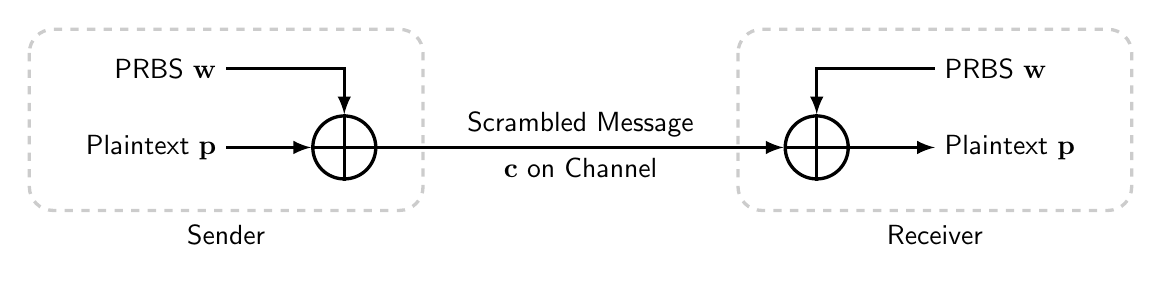
\begin{tikzpicture}[font=\sffamily]
		% input xor
		\node (inxor) at (0cm, 0cm) [very thick, circle, draw, minimum height = 0.8cm, minimum width = 0.8cm] {};
		\draw [very thick] (inxor.north) -- (inxor.south);
		\draw [very thick] (inxor.east) -- (inxor.west);

		% output xor
		\node (outxor) at (6cm, 0cm) [very thick, circle, draw, minimum height = 0.8cm, minimum width = 0.8cm] {};
		\draw [very thick] (outxor.north) -- (outxor.south);
		\draw [very thick] (outxor.east) -- (outxor.west);

		\draw [very thick, -latex] (inxor.east) -- (outxor.west) node [pos=.5, above] {Scrambled Message} node [pos=.5, below] {$\mathbf c$ on Channel};

		\node [anchor = east] (inplain) at (-1.5cm, 0cm) {Plaintext $\mathbf p$};
		\draw [very thick, -latex] (inplain.east) -- (inxor.west);

		\node [anchor = east] (inprbs) at (-1.5cm, 1cm) {PRBS $\mathbf w$};
		\draw [very thick, -latex] (inprbs.east) -| (inxor.north);

		\node [anchor = west] (outprbs) at (7.5cm, 1cm) {PRBS $\mathbf w$};
		\draw [very thick, -latex] (outprbs.west) -| (outxor.north);

		\node [anchor = west] (outplain) at (7.5cm, 0cm) {Plaintext $\mathbf p$};
		\draw [very thick, -latex] (outxor.east) -- (outplain.west);

		\draw [very thick, rounded corners = 0.3cm, dashed, color = black!20!white] (-4cm, 1.5cm) rectangle (1cm, -0.8cm) node[color = black, pos=.5, below = 1.2cm] {Sender};

		\draw [very thick, rounded corners = 0.3cm, dashed, color = black!20!white] (5cm, 1.5cm) rectangle (10cm, -0.8cm) node[color = black, pos=.5, below = 1.2cm] {Receiver};
	\end{tikzpicture}
	\caption{Basic principle of scrambling / descrambling, loosely based on \cite[Figure 7.20]{dspfpga}}
	\label{fig:scrambling_principle}
\end{figure}

\subsection{Implementation by Sigfox}
The \gls{ecc}, payload, \gls{mac} tag and \gls{crc} segments of every downlink frame are scrambled.
\Cref{fig:downlink_scrambler} shows a schematic diagram for the scrambler used by Sigfox.
Since scrambling and descrambling are equivalent operations (both perform a bitwise XOR with the same \gls{prbs}), the same schematic can also be used to descramble a received frame at the receiver.

\xblackout{This section about the downlink's scrambling algorithm has been removed, sorry :(
removed removed removed removed removed removed removed removed removed removed removed
removed removed removed removed removed removed removed removed removed removed removed
removed removed removed removed removed removed removed removed removed removed removed
removed removed removed removed removed removed removed removed removed removed removed
removed removed removed removed removed removed removed removed removed removed removed
removed removed removed removed removed removed removed removed removed removed removed
removed removed removed removed removed removed removed removed removed removed removed}

\begin{figure}[h]
	\centering
	\censorbox*[\small]{80}{15}{1}
	\caption{Schematic diagram of scrambler / descrambler for Sigfox-specific downlink whitening}
	\label{fig:downlink_scrambler}
\end{figure}

\subsection{Open Implementation}
\label{sec:downlink_scrambling_reimp}
\xblackout{This section about the downlink's scrambling algorithm has been removed, sorry :(
removed removed removed removed removed removed removed removed removed removed removed
removed removed removed removed removed removed removed removed removed removed removed
removed removed removed removed removed removed removed removed removed removed removed
removed removed removed removed removed removed removed removed removed removed removed
removed removed removed removed removed removed removed removed removed removed removed
removed removed removed removed removed removed removed removed removed removed removed
removed removed removed removed removed removed removed removed removed removed removed
removed removed removed removed removed removed removed removed removed removed removed
removed removed removed removed removed removed removed removed removed removed removed
removed removed removed removed removed removed removed removed removed removed removed
removed removed removed removed removed removed removed removed removed removed removed
removed removed removed removed removed removed removed removed removed removed removed
removed removed removed removed removed removed removed removed removed removed removed
removed removed removed removed removed removed removed removed removed removed removed
removed removed removed removed removed removed removed removed removed removed removed
removed removed removed removed removed removed removed removed removed removed removed}

\subsection{Result}
The Open Implementation of scrambler / descrambler not only achieves feature parity with Sigfox's implementation, but even makes it possible to descramble frames without prior knowledge about corresponding uplink \gls{sn} or target device ID.
The descrambler in \texttt{librenard} was tested with downlinks from the two base stations in \Cref{fig:basestation_photo} and the scrambler was tested by sending multiple forged downlinks to the \textit{Pycom SiPy}.

It is not evident why Sigfox chose to implement scrambling in their downlink protocol, especially \xblackout{removed removed removed removed removed removed removed removed removed removed removed}.
Possibly, scrambling is not only used as a technique that simplifies synchronization at the receiver side, but also as zero-overhead method for the Sigfox object to discriminate downlink frames.
Theoretically, two Sigfox objects could request downlink frames from a base station at the same frequency at approximately the same time.
In that case, the protocol requires the base station to send downlinks to both objects, which are both listening simultaneously.
The downlink frame does not contain any field to target the downlink message at only one of the two objects (e.g. a ``device ID'' field is missing).
Thus, by seeding the scrambler with a value that is also derived from the device ID, it is made sure that if the wrong Sigfox object receives the downlink, descrambling and thus the \gls{crc} check will likely fail.
\xblackout{This section about the downlink's scrambling algorithm has been removed, sorry :(}
Any Sigfox object, upon receiving a downlink, should check the contained \gls{mac} tag anyway.
Unless the object was actually the target of the downlink, this check should fail with a very high probability ($\frac{2^{16} - 1}{2^{16}}$) since the \gls{mac} tag depends on every object's unique \gls{nak}.
Therefore, generating \gls{prbs} based on device ID and \gls{sn} is not technically necessary for the functioning of the downlink protocol.

A second, more daring theory is that downlink scrambling may be part of a ``security by obscurity'' scheme, that should make it harder for adversaries that eavesdrop on a downlink transmission to gain knowledge about its contents.
Two observations that support this thesis is that the seed is not only based on the device ID, but also on the uplink \gls{sn}, which no justifiable reason seems to exist for and also the fact that a very unusual scrambler architecture \censor{removed removed removed} is employed.
However, as the work of the previous section shows, there is no notable secrecy gained through scrambling \censor{removed removed removed}.
Thus, if the objective of scrambling is security, it can be deemed useless in that regard.

\FloatBarrier
\section{Preliminary Security Assessment}
In general, the promises made by Sigfox concerning the security of their downlink \cite[Section 2.2]{sigfox_security_whitepaper} are met.

For example, Sigfox claims that the authenticity of all messages, thus also that of downlink messages, is verified by the receiving Sigfox object, just like the base station checks the authentication information of uplinks.
This claim has been tested and shown to be correct, at least in the case of the \textit{Pycom SiPy}.
However, all three methods (waiting for \gls{sn} overflow, obtaining a \gls{nak} through physical access, guessing a valid \gls{mac} tag) to possibly break message authentication described when assessing the uplink's security (\Cref{sec:uplink_security}) also apply to the downlink.
Since Sigfox objects only listen for downlinks during a short interval after transmitting an uplink, the chance of successfully guessing a \gls{mac} tag is diminished though.

In \Cref{sec:downlink_scrambling_reimp}, it has been shown that scrambling of the downlink frame does not provide any protection against eavesdropping, so Sigfox users should not expect confidentiality of the downlink's payload.
On the other hand, reversing the scrambling and making it possible to read the payload in plain does not imply that authenticity checking is broken at all.
In fact, the authentication mechanism using a \gls{mac} tag is completely independent from scrambling.

One key weakness of the downlink protocol is its susceptibility to intentional jamming or unintentional interference, allowing \gls{dos}-style attacks.
For example, transmitters for the European 869.4 MHz to 869.65 MHz \gls{srd} band are easy to obtain and operate, even for the layperson.
Since Sigfox objects only listen for downlinks during a short interval, any radio interference at the downlink's frequency during this interval inhibits the accurate reception of the downlink frame.
Theoretically, an attacker could deliberately induce radio interference by transmitting at the right frequency at the right time.
While jamming itself is usually illegal, a suitable transmitter could still conform to statutory regulations and would be hard to track down.
Therefore, the downlink should not be used to transmit safety or security-critical data to \gls{iot} devices and device makers should not rely on the downlink's dependability.
